% !TeX program = lualatex
% !TeX root = luaking.tex
% !TeX encoding = UTF-8
% !TeX spellcheck = cs_CZ
%---------------------------------------------------------------------------------------------------
% file fey1ch21.tex
%---------------------------------------------------------------------------------------------------
%=========================== Kapitola: Harmonický oscilátor ========================================
\setchaptertoc
\chapter{Harmonický oscilátor}\label{fyz:IchapXXI}
  \section{Lineární diferenciální rovnice}\label{fyz:IchapXXIsecI}
    Kurz studia fyziky se obvykle dělí na tématické části jako například mechanika, elektřina,
    optika atd., přičemž se studují jedna za druhou. Například v našem kurzu jsme se zatím většinou
    zabývali mechanikou. Znovu a znovu se však stává podivná věc: rovnice, jež se objevují v různých
    odvětvích fyziky, a dokonce i v jiných vědách, jsou často téměř stejné. Mnohé jevy mají proto
    své analogie v těchto různých odvětvích. Jako jednoduchý příklad uveďme, že šíření zvukových vln
    je v mnohém podobné šíření světelných vln. Při podrobném studiu akustiky zjistíme, že studujeme
    téměř totéž, jako kdybychom se podrobně zabývali studiem optiky. Studium nějakého jevu v jedné
    oblasti tak může rozšířit naše vědomosti v jiné oblasti. Nejlépe bude, když si od začátku
    uvědomíme, že takováto rozšíření jsou možná, neboť jinak by možná někdo neviděl důvod, proč
    ztrácet čas a energii s něčím, co se zdá být jen malou částí mechaniky.
    
    Harmonický oscilátor, který se chystáme studovat, má blízké analogie v mnoha jiných odvětvích.
    Ať už začneme s příkladem závaží na pružině, kyvadla s malou výchylkou nebo jiných mechanických
    zařízení, studujeme ve skutečnosti určitou \textbf{diferenciální rovnici}. Tato rovnice se ve
    fyzice i v jiných vědách objevuje vždy znovu a znovu. Ve skutečnosti je částí tolika jevů, že
    její studium si zaslouží naši pozornost. Některé jevy, které popisuje tato rovnice, jsou
    oscilace tělesa na pružině, oscilace náboje v elektrickém obvodu, oscilace ladičky vytvářející
    zvukové vlny, vibrace elektronů v atomu vytvářející světelné vlny, rovnice činnosti takového
    servosystému, jakým je termostat regulující teplotu, komplikované interakce v chemických
    reakcích, růst kolonie bakterií interagujících s dodávanou potravou a otravnými látkami, které
    bakterie produkují, lišky, požírající králíky žeroucí trávu atd. Všechny tyto jevy probíhají
    podle rovnic, jež jsou si velmi podobné, a to je důvod, proč se tak podrobně zabýváme
    mechanickým oscilátorem. Tyto rovnice jsou \textbf{lineárními diferenciálními rovnicemi s
    konstantními koeficienty}. Lineární diferenciální rovnice s konstantními koeficienty je rovnice,
    která se skládá ze součtu více členů, přičemž každý člen je derivací závisle proměnné podle
    nezávisle proměnné vynásobený nějakou konstantou. Takže
    \begin{equation}\label{fyz:eq727}
      a_n\diff[n]xt +a_{n−1}\diff[n-1]xt +\cdots+a_1\diff{x}{t}+a_0x = f(t)
    \end{equation}
    se nazývá lineární diferenciální rovnicí \(n\)-tého řádu s konstantními koeficienty (každé
    \(a_i\) je konstanta). Podrobně se obyčejným diferenciálním rovnicím věnuje kapitola
    \ref{vol01:mai:IIchapIV}. 

  \section{Harmonický oscilátor}\label{fyz:IchapXXIsecII}
    Snad nejjednodušším mechanickým systémem, který se při svém pohybu řídí lineární diferenciální
    rovnicí s konstantními koeficienty, je těleso zavěšené na pružině. Pružina se nejdříve napne,
    aby vyvážila tíhu tělesa. Když nastane rovnováha, zajímáme se o vertikální výchylky tělesa z
    rovnovážné polohy (obr. \ref{fyz:fig0246}). Posunutí směrem nahoru označíme \(x\) a budeme
    předpokládat, že pružina je dokonale lineární. V takovém případě síla, jíž působí pružina, když
    ji natáhneme, je přímo úměrná výchylce, tj. síla je rovna \(-kx\) (se znaménkem mínus, neboť
    síla působí opačným směrem než posunutí). Takže hmotnost tělesa krát jeho zrychlení je rovno
    \(-kx\)
    \begin{equation}\label{fyz:eq728}
      m\diff[2]xt = -kx
    \end{equation}
    Pro jednoduchost předpokládejme (nebo můžeme vhodně změnit jednotky času), že podíl
    \(k/m =1\). Nejdříve se budeme zabývat rovnicí
    \begin{equation}\label{fyz:eq729}
      \diff[2]xt = -x,
    \end{equation}
    ale později se vrátíme k rovnici (\ref{fyz:eq728}) s explicitně zapsanými \(k\) a \(m\).
    \begin{figure}[ht!] %\ref{fyz:fig0246}
      \centering
      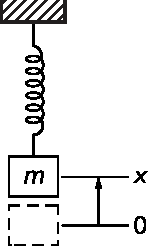
\includegraphics[width=0.3\linewidth]{fyz_fig0246.pdf}
      \caption{Těleso upevněné na pružině - jednoduchý příklad harmonického oscilátoru
               (\cite[s.~287]{Feynman01})}
      \label{fyz:fig0246}
    \end{figure}
    Numerickou analýzu rovnice (\ref{fyz:eq729}) jsme provedli již tehdy, kdy jsme se poprvé začali
    zabývat mechanikou. Tuto rovnici (\ref{fyz:eq129}) jsme řešili, abychom našli pohyb. Pomocí
    numerické integrace jsme dostali křivku (obr. \ref{fyz:fig0102}), podle níž, bylo-li \(m\) na
    začátku vychýleno, ale jinak v klidu, se začne pohybovat směrem dolů a projde nulovou polohou.
    Dále jsme jeho pohyb nesledovali, ale samozřejmě víme, že se pohybuje směrem nahoru a dolů - že
    \emph{osciluje}. Při numerických výpočtech jsme zjistili, že rovnovážnou polohou prošla křivka v
    bodě \(t= \num{1.570}\). Délka celého cyklu je čtyřikrát větší, \(T_0 =\SI{6.28}{\s}\) „s“ (v
    našich časových jednotkách). To jsme zjistili numericky, dokud jsme ještě neznali infinitezimální
    počet. Předpokládáme, že mezi tím nás na v kurzu \ref{vol01:mai:IchapV} z matematiké analýzy
    seznámili s funkcí, která se po dvojnásobném derivování zreprodukuje se znaménkem mínus.
    (Samozřejmě, existují způsoby, jak tuto funkci najít přímo, ale ty jsou složitější, než když
    řešení jednoduše přijmeme.) jde o \(x=\cos t\). Zderivujeme-li ji, najdeme \(\diff{x}{t} = -\sin
    t\) a \(\diff[2]xt=-\cos t=-x\). Funkce \(x=\cos t\) má v bodě \(t= 0\) počáteční hodnotu
    \num{1} a počáteční rychlost je rovna nule. S takovými počátečními podmínkami jsme začínali naši
    numerickou analýzu. Nyní, když víme, že \(x=\cos t\), můžeme vypočítat přesnou hodnotu času, za
    který projde bodem \(x=0\). Odpověď je: \(t=\frac{\pi}{2}\) nebo \num{1.57108}. V důsledku chyb
    při numerické analýze jsme se zmýlili v poslední číslici, ale byla to velmi blízká hodnota!

    Abychom se dostali dále při řešení problémů, vrátíme se s jednotkami času ke skutečným sekundám.
    Jaké je potom řešení? Na začátku se můžeme domnívat, že konstanty \(k\) a \(m\) se nám podaří
    zahrnout, jestliže \(\cos t\) něčím vynásobíme. Zkusme tedy \(x=A\cos t\). Potom \(\diff{x}{t}=
    -A\sin t\) a \(\diff[2]xt = -A\cos t= - x\).

    K našemu překvapení vidíme, že jsme neuspěli v řešení rovnice (\ref{fyz:eq728}), ale znovu jsme
    dostali rovnici (\ref{fyz:eq729})! Tato skutečnost je ilustrací jedné z nejdůležitějších
    vlastností lineárních rovnic: \emph{Vynásobíme-li nějaké řešení libovolnou konstantou, dostaneme
    znovu řešení téže rovnice.} Matematický důvod je jasný. Je-li \(x\) řešením a vynásobíme-li obě
    strany rovnice \(A\), pak všechny derivace jsou vynásobeny \(A\), a proto \(Ax\) je právě tak
    dobré řešení, jako bylo \(x\). Fyzikální důvod je takový: Stáhneme-li závaží zavěšené na pružině
    dolů dvakrát tak daleko než dříve, síla je dvojnásobná, výsledné zrychlení je dvojnásobné,
    rychlost získaná za danou dobu je dvojnásobná a vzdálenost prošlá za danou dobu je dvojnásobná.
    Ale těleso \emph{musí} projít dvojnásobnou vzdálenost, aby se dostalo zpět do počátku, protože
    jsme ho na začátku vychýlili dvakrát tak daleko. Takže do počátku se vrátí za stejnou dobu, bez
    ohledu na velikost počáteční výchylky. Jinými slovy: Pohyb popsaný lineární rovnicí má stejný
    \emph{časový průběh} bez ohledu na to, jak velkou silou byl vyvolán.

    Neprovedli jsme správnou úpravu - jen jsme se poučili, že řešení můžeme vynásobit jakoukoli
    konstantou a bude vyhovovat stejné rovnici, avšak ne jiné rovnici. Po takovýchto pokusech s
    násobením \(x\) nějakou konstantou zjišťujeme, že musíme změnit časově měřítko. Jinak řečeno,
    rovnice (\ref{fyz:eq728}) má řešení ve tvaru
    \begin{equation}\label{fyz:eq730}
      x=\cosω_0t.
    \end{equation}
    (Je důležité si uvědomit, že v tomto případě \(\omega_0\) není úhlovou rychlostí rotujícího
    tělesa, ale kdybychom nesměli použít stejné písmeno k označení více než jedné věci, neměli
    bychom dost písmen.) Důvod, proč jsme označili \(\omega\) indexem nula je ten, že za chvíli
    budeme mít více symbolů \(\omega\). Zapamatujme si, že \(\omega_0\) odpovídá přirozenému pohybu
    oscilátoru. Nyní zkusme dosadit do rovnice (\ref{fyz:eq730}). Jsme na tom lépe, neboť
    \(\diff{x}{t}=−ω_0\sinω_0t\) a
    \begin{equation*}
      \diff[2]xt = −ω^2_0\cosω_0t = −ω^2_0x
    \end{equation*}
    Takže na konec jsme přece jen vyřešili rovnici, kterou jsme chtěli řešit. Rovnice \(\diff[2]xt =
    −ω^2_0x\) je stejná jako rovnice (\ref{fyz:eq727}), jestliže \(\omega_0^2 = k/m\).

    Dále musíme prozkoumat fyzikální význam \(ω_0\). Víme, že funkce kosinus se opakuje s periodou
    \(2\pi\). Takže \( x=\cosω_0t\) bude opakovat stejný pohyb (projde celým cyklem), změní-li se
    „úhel“ o \(2\pi\). Veličina \(ω_0t\) se často nazývá \textbf{fází pohybu}. Abychom změnili
    \(ω_0t\) o \(2π\), musí se čas změnit o hodnotu \(T_0\), která se nazývá \textbf{periodou} jedné
    úplné oscilace. Samozřejmě musí platit, že \(\omega_0T_0 = 2\pi\), tj. \(\omega_0T_0\) musí
    odpovídat jednomu cyklu úhlové proměnné a všechno se zopakuje, zvětšíme-li \(t\) o \(T_0\) a
    fázi o \(2\pi\). Takže
    \begin{equation}\label{fyz:eq731}
      t_0=\frac{2π}{ω_0}=2π\sqrt{\frac{m}{k}}
    \end{equation}  
    Budeme-li mít těžší závaží, budou oscilace pružiny trvat déle. Je to proto, že závaží má větší
    setrvačnou hmotnost a protože síly jsou stejné, potrvá déle, než se závaží rozhýbe. Bude-li
    pružina silnější, bude pohyb rychlejší, a to souhlasí: Je-li pružina silnější, perioda se
    zkracuje.

    Všimněme si, že perioda kmitu závaží na pružině nezávisí na tom, jak pohyb začal, jak daleko
    pružinu vychýlíme. \emph{Perioda} oscilací je určena rovnicí pohybu (\ref{fyz:eq728}), ale není
    jí určena amplituda. Ta je určena tím, jak pohyb začneme, tím čemu říkáme \textbf{počáteční
    podmínky}.

    Ve skutečnosti jsme ještě nenašli nejobecnější možné řešení rovnice (\ref{fyz:eq727}). Existují
    i jiná řešení. Je jasné proč - všechny případy popsané \(x = a \cos\omega_0 t\) začínají s
    počátečním posunutím a nulovou počáteční rychlostí. Ale pohyb například může začít, když je
    \(x=0\) a tělesu dodáme úderem rychlost v čase \(t= 0\). Takový pohyb není popsán kosinem, ale
    sinem. Jinak lze problém formulovat i takto: Je-li \(x = \cos\omega_0 t\) řešením, pak není
    zřejmé, zda bude pohyb stejný i tehdy, kdy náhodou vejdeme do místnosti v nějakém okamžiku
    (který nazveme „\(t= 0\)“) a uvidíme těleso jak právě prochází polohou \(x= 0\). Proto \(x =
    \cos\omega_0 t\) nemůže být nejobecnějším řešením, musí být možné posunout začátek času. Jako
    příklad můžeme řešení napsat takto: \(x = a \cos\omega_0(t - t_1)\), kde \(t_1\) je nějaká
    konstanta. To odpovídá posunutí začátku času do nějakého jiného okamžiku. Dále můžeme psát
    \begin{equation*}
      \cos(ω_0t+Δ) = \cosω_0t\cosΔ−\sinω_0t\sinΔ,
    \end{equation*}
    a
    \begin{equation*}
      x = A\cosω_0t+B\sinω_0t,
    \end{equation*}
    kde \(A=a\cosΔ\) a \(B=−a\sinΔ\). Libovolný z těchto tvarů lze použít k zápisu obecného řešení
    rovnice (\ref{fyz:eq727}), tj. každé řešení diferenciální rovnice \(\diff[2]xt=−ω^2_0x\), které
    existuje, lze napsat jako
    \begin{subequations}\label{fyz:eq732}
      \begin{align}
        x=a\cosω_0(t−t_1),        \label{fyz:eq732a}\\
        x=a\cos(ω_0t+Δ),          \label{fyz:eq732b}\\
        x=A\cosω_0t+B\sinω_0t.    \label{fyz:eq732c}
      \end{align}
    \end{subequations}

    Některé veličiny v (\ref{fyz:eq732}) mají svůj název: \(\omega_0\) se nazývá \textbf{úhlovou
    frekvencí}; je to počet radiánů, o které se fáze změní za sekundu. Je určena diferenciální
    rovnicí. Ostatní konstanty nejsou určeny diferenciální rovnicí, ale počátečními podmínkami. Z
    těchto konstant udává \(a\) maximální dosaženou výchylku a nazývá se \textbf{amplitudou kmitů}.
    Konstantě \(A\) se někdy říká \textbf{fáze} oscilací, ale to je nedorozumění, neboť jinak se
    fází nazývá \(\omega_0t + \Delta\) , přičemž se fáze mění v závislosti na čase. \(\Delta\)
    můžeme nazvat \textbf{fázovým posunem} od nějaké definované nulové fáze. Řekněme to jinak - různá
    \(\Delta\) odpovídají pohybům v různých fázích. Tak je to správně, ale jestli si můžeme nebo
    nemůžeme dovolit nazvat \(\Delta\) fází, to je jiná otázka.

  \twocolumn[\section{Harmonický pohyb a pohyb po kružnici}\label{fyz:IchapXXIsecIII}]
    Skutečnost, že řešení rovnice (\ref{fyz:eq728}) obsahuje kosinus, svědčí o tom, že tu může být
    nějaká souvislost s kružnicemi. Samozřejmě, je to umělá souvislost, neboť v lineárním pohybu se
    kružnice nevyskytují - je to prostě pohyb sem a tam. Mohli bychom poukázat na to, že tuto
    diferenciální rovnici jsme vlastně již vyřešili při studiu mechaniky pohybu po kružnici.
    Vykonává-li částice pohyb po kružnici konstantní rychlostí \(v\), otáčí se polohový vektor
    spojující střed kružnice s částicí o úhel, jehož velikost se zvětšuje úměrně s časem. Nazveme-li
    tento úhel \(θ=vt/R\) (obr. \ref{fyz:fig0247}), pak \(\diff{θ}{t}=ω_0= v/R\). Přitom působí
    dostředivé zrychlení \(a=v^2/R= ω^2_0R\). V jakémkoli okamžiku je souřadnice \(x\) rovna
    poloměru krát \(\cosθ\) a souřadnice \(y\) je rovna součinu poloměru a \(\sinθ\):
    \begin{equation*}
      x=R\cosθ,\qquad y=R\sinθ.
    \end{equation*}
    \begin{figure}[ht!] %\ref{fyz:fig0247}
      \centering
      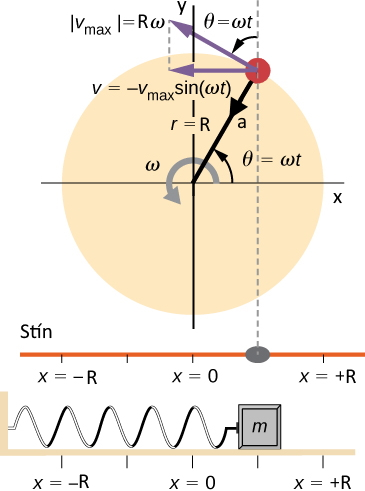
\includegraphics[width=0.8\linewidth]{fyz_fig0247_ver1.jpg}
      \caption{Částice pohybující se po kruhové dráze konstantní rychlostí
              (\cite[s.~290]{Feynman01})}
      \label{fyz:fig0247}
    \end{figure}
    A co se zrychlením? Čemu je rovna \(x\)-ová složka zrychlení \(\diff[2]xt=\)? Geometricky jsme
    si již odvodili, že je rovna velikostí zrychlení vynásobené kosinem prošlého úhlu se záporným
    znaménkem, neboť směřuje do středu
    \begin{equation}\label{fyz:eq733}
      a_x=−a\cosθ=−ω^2_0R\cosθ=−ω^2_0x.
    \end{equation}

    Jinak řečeno, koná-li částice pohyb po kružnici, má horizontální složka pohybu zrychlení, jež je
    úměrné horizontální vzdálenosti od středu. Samozřejmě známe i řešení pohybu po kružnici:
    \(x=R\cosω_0t\). Rovnice (\ref {fyz:eq733}) nezávisí na poloměru kružnice, proto pro jakoukoli
    kružnici máme stejné řešení při daném \( ω_0\). Na základě různých důvodů můžeme očekávat, že
    velikost výchylky závaží na pružině bude úměrná \(\cosω_0t\) a bude to představovat stejný
    pohyb, jaký bychom viděli, kdybychom se dívali na \(x\)-ovou složku polohy tělesa obíhajícího po
    kružnici úhlovou rychlostí \( ω_0\).  Jako důkaz lze experimentálně ověřit, že pohyb závaží
    zavěšeného na pružině směrem nahoru a dolů je při pohledu ze strany stejný jako pohyb po
    kružnici. Na obr. \ref{fyz:fig0248} se stíny knoflíku na klice kola a závaží svisle kmitajícího na
    pružině pohybují souběžně. Rozkmitáme-li závaží ve správném okamžiku ze správné polohy a jsou-li
    obrátky kola nastaveny tak, aby frekvence obou pohybů souhlasily, pak se budou oba stíny
    pohybovat současně. Stejně lze porovnat numerické řešení, které jsme našli předtím s funkcí
    kosinus a přesvědčit se, zda souhlasí.

    \begin{figure}[ht!] %\ref{fyz:fig0248}
      \centering
      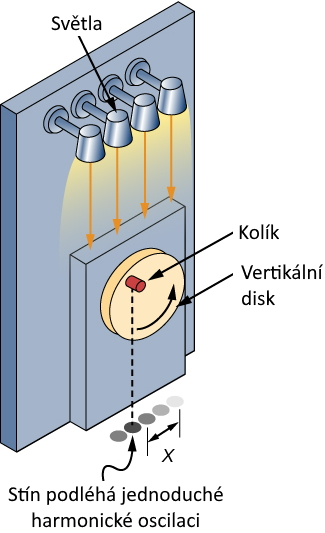
\includegraphics[width=0.8\linewidth]{fyz_fig0248_ver1.jpg}
      \caption{Demonstrace ekvivalence jednoduchého harmonického pohybu a rovnoměrného pohybu po 
              krunici
              (\cite[s.~290]{Feynman01})}
      \label{fyz:fig0248}
    \end{figure}

    Na tomto místě můžeme poznamenat, že když je rovnoměrný pohyb po kružnici tak úzce spjat s
    kmitavým pohybem, můžeme kmitavý pohyb popsat jednodušeji jako projekci pohybu hmotného bodu po
    kružnici. Jinak řečeno, i když vzdálenost \(y\) v případě oscilátoru nemá význam, můžeme rovnici
    (\ref{fyz:eq728}) napsat i pro \(y\) a obě rovnice spojit. To nám umožní provést analýzu našeho
    jednorozměrného oscilátoru pomocí znalostí pohybů po kružnici, což je mnohem snadnější, než
    kdybychom museli řešit příslušnou diferenciální rovnici. To lze provést použitím komplexních
    čísel, což si ukážeme v následující kapitole.

  \section{Počáteční podmínky}\label{fyz:IchapXXIsecIV}
    Nyní se zamysleme nad tím, co určuje konstanty \(A\) a \(B\) nebo \(a\) a \(\Delta\). Tyto
    konstanty jsou určeny tím, jak začne pohyb. Uvedeme-li závaží do pohybu tak, že ho trochu
    vychýlíme, máme jeden druh oscilací. Vychýlíme-li ho nejdříve a při pouštění postrčíme,
    dostaneme zase jiný pohyb. Konstanty \(A\) a \(B\) nebo \(a\) a \(\Delta\) jsou určeny tím, jak
    pohyb začal a ničím jiným, tj. takzvanými \textbf{počátečními podmínkami}. Ukážeme si, jak
    počáteční podmínky souvisí s těmito konstantami. Ačkoli bychom k tomu mohli použít jakýkoli z
    tvarů (\ref{fyz:eq732}), nejsnadnější to je s tvarem (\ref{fyz:eq732c}). Předpokládejme, že v
    čase \(t=0\) jsme pohyb začali s počáteční výchylkou \(x_0\) a rychlostí \(v_0\). To je
    nejobecnější způsob, jak může pohyb začít. (Počáteční \emph{zrychlení} nemůžeme zadat, neboť to
    je dáno vlastností pružiny, jakmile známe \(x_0\)). Nyní vypočítejme \(A\) a \(B\). Začneme s
    rovnicí pro \(x\)
    \begin{equation*}
      x=A\cosω_0t+B\sinω_0t.
    \end{equation*}
    Protože později budeme potřebovat i rychlost, zderivujeme \(x\) a dostaneme
    \begin{equation*}
      v=−ω_0A\sinω_0t+ω_0B\cosω_0t.
    \end{equation*}
    Tyto vztahy platí pro každé \(t\), ale my známe \(x\) a \(v\) v okamžiku \(t=0\). Dosadíme-li do
    těchto rovnic \(t=0\), na levé straně budeme mít \(x_0\) a \(v_0\), tj. hodnoty pro \(x\) a
    \(v\) v okamžiku \(t=0\). Víme, že kosinus nuly je jedna a sinus nuly je nula, a tak
    \begin{equation*}
      x_0=A⋅1+B⋅0=A
    \end{equation*}
    a
    \begin{equation*}
      v_0=−ω_0A⋅0+ω_0B⋅1=ω_0B.
    \end{equation*}
    takže pro tento zvláštní případ platí
    \begin{equation*}
      A=x_0,\qquad B=v_0/ω_0.
    \end{equation*}
    Z hodnot \(A\) a \(B\) můžeme vypočítat \(a\) a \(\Delta\), chceme-li.

    Tím máme problém vyřešen, ale je tu ještě jedna fyzikálně zajímavá věc, kterou bychom měli
    ověřit, a to zachování energie. Protože nedochází ke ztrátám třením, energie by se měla
    zachovávat. Použijeme vztahy
    \begin{align*}
      x&=a\cos(ω_0t+Δ);   \\
      \shortintertext{pak}
      v&=−ω_0a\sin(ω_0t+Δ).
    \end{align*}
    Vypočítejme kinetickou \(T\) a potenciální energii \(U\). Potenciální energie v kterémkoli
    okamžiku je \(1/2kx^2\), kde \(x\) je výchylka a \(k\) tuhost pružiny. Dosadíme-li za \(x\),
    máme
    \begin{equation*}
      U=\frac{1}{2}kx^2=\frac{1}{2}ka^2\cos^2(ω_0t+Δ).
    \end{equation*}
    je vidět, že potenciální energie není konstantní. Nikdy není záporná, což je přirozené, neboť
    v pružině je vždy nějaká energie, ale její velikost se mění s \(x\). Na druhé straně, kinetická
    energie je rovna \(\frac{1}{2}mv^2\) a dosazením za \(v\) máme
    \begin{equation*}
      T=\frac{1}{2}mv^2=\frac{1}{2}mω^2_0a^2\sin^2(ω_0t+Δ).
    \end{equation*}
    Pro maximální \(x\) je kinetická energie rovna nule, neboť rychlost je nulová, a v okamžiku, kdy
    \(x\) prochází nulou, je kinetická energie maximální, neboť tehdy je pohyb nejrychlejší. Tyto
    změny kinetické energie jsou právě opačné než změny potenciální energie, ale celková energie
    musí být konstantní. Když si všimneme, že \(k= m\omega^2_0\), vidíme, že
    \begin{align*}
      T+U&=\frac{1}{2}mω^2_0a^2[\cos^2(ω_0t+Δ)+\sin^2(ω_0t+Δ)]      \\
         &=\frac{1}{2}mω^2_0a^2.
    \end{align*}
    Energie je úměrná druhé mocnině amplitudy. Zdvojnásobí-li se amplituda, zvětší se energie
    čtyřnásobně. Střední potenciální energie je rovna polovině celkové energie a střední kinetická
    energie je podobně rovna polovině celkové energie.

  \section{Nucené kmity}\label{fyz:IchapXXIsecV}
    V dalším textu se budeme zabývat \emph{harmonickým oscilátorem s nucenými kmity}, tj. takovým,
    na který působí vnější budicí síla. Rovnice takového oscilátoru je
    \begin{equation}\label{fyz:eq734}
      m\diff[2]xt=−kx+F(t).
    \end{equation}
    Rádi bychom zjistili, co se bude dít za takových okolností. Vnější budicí síla může mít různé
    závislosti na čase. První závislost, jíž se budeme zabývat, je velmi jednoduchá - budeme
    předpokládat, že síla se mění harmonicky
    \begin{equation}\label{fyz:eq735}
      F(t)=F_0\cosωt.
    \end{equation}
    Všimněme si však, že toto \(\omega\) se nemusí rovnat \(\omega_0\): máme pod svou kontrolou -
    buzení může mít různé frekvence. Rovnici (\ref{fyz:eq734}) se pokusíme vyřešit pro zvláštní sílu
    (\ref{fyz:eq735}). Jaké řešení má rovnice (\ref{fyz:eq734})? Jedním partikulárním řešením
    (obecnější případ si probereme později) je
    \begin{equation}\label{fyz:eq736}
      x=C\cosωt,
    \end{equation}
    kde je třeba určit \(C\) jinak řečeno, můžeme předpokládat, že nutí-li vnější síla těleso
    pohybovat se sem a tam, pak těleso sleduje působení síly. Ať už je to jakkoli, můžeme to zkusit.
    Dosadíme (\ref{fyz:eq736}) do (\ref{fyz:eq734}) a máme
    \begin{equation*}
      −mω^2C\cosωt=−mω^2_0C\cosωt+F_0\cosωt.
    \end{equation*}
    Dosadili jsme i \(k=mω^2_0\), abychom této rovnici nakonec lépe porozuměli. Protože v každém
    členu je \(\cos\omega t\), můžeme jím rovnici vydělit a vidíme, že (\ref{fyz:eq736}) je skutečně
    řešením, za předpokladu, že \(C\) zvolíme Správně. \(C\) musí být rovno
    \begin{equation}\label{fyz:eq738}
      C=\frac{F_0}{m(ω^2_0−ω^2)}.
    \end{equation}
    tj. částice \(m\) kmitá se stejnou frekvencí jako síla, ale s amplitudou, která závisí na
    frekvenci budicí síly a na vlastní frekvenci oscilátoru. Za prvé to znamená, že je-li \(\omega\)
    velmi malé ve srovnání s \(\omega_0\), pak posunutí a síla mají stejný směr. Na druhé straně,
    když budeme závaží nutit kmitat velmi rychle, pak (\ref {fyz:eq738}) nám říká, že \(C\) je
    záporné pro \(\omega\) větší než vlastní frekvence oscilátoru \(\omega_0\) (\(\omega_0\) budeme
    nazývat vlastní frekvencí harmonického oscilátoru a \(\omega\) budící frekvencí). Při velmi
    vysoké frekvenci může být jmenovatel velmi velký a amplituda je potom velmi malá.

    Samozřejmě, řešení, které jsme našli, je vyhovujícím řešením, jen od určitého časového počátku,
    neboť jinak existuje i takové řešení, které se po chvíli utlumí. Toto druhé řešení se nazývá
    \textbf{přechodovou odezvou} na \(F(t)\), zatímco (\ref{fyz:eq736}) a (\ref{fyz:eq738}) se
    nazývají \textbf{ustálenou odezvou}.

    Podle našeho vztahu (\ref{fyz:eq738}) by se měl vyskytovat pozoruhodný jev: Je-li \(\omega\)
    téměř stejné jako \(\omega_0\), blíží se \(C\) k nekonečnu. Proto nastavíme-li frekvenci vnější
    síly tak, aby byla v souladu s vlastní frekvencí, měli bychom dostat mimořádně velké výchylky.
    To ví dobře každý, kdo houpal dítě na houpačce. Nešlo by nám to, kdybychom zavřeli oči a
    houpačku rozhoupávali libovolně určitou frekvencí. Podaří-li se nám najít správný rytmus, létá
    houpačka velmi vysoko, máme-li však špatný rytmus, můžeme někdy tlačit, kdybychom správně měli
    táhnout a podobně - prostě to nejde.

    Nastavíme-li \(\omega\) tak, aby bylo přesně rovno \(\omega_0\), měla by být amplituda
    oscilátoru nekonečná, což je nemožné. Příčinou je to, že naše rovnice tehdy přestane platit.
    Projeví se dodatečné členy, které odpovídají tření a dalším silám, jež nejsou v rovnici
    (\ref{fyz:eq734}) zahrnuty, ale které se vyskytují v reálném světě. Proto se amplituda nezvětší
    z nějakého důvodu do nekonečna. Například proto, že pružina praskne!

  \section{Příklady a cvičení}\label{fyz:IchapXXIsecVI}

%---------------------------------------------------------------------------------------------------